\documentclass[12pt, oneside]{book}
% This provides the \BibTeX macro
\usepackage{doc}
\usepackage{makeidx}

\usepackage[tight,footnotesize]{subfigure}
\usepackage{amsmath}
\usepackage{amsfonts}

\newtheorem{problem}{Problem}
\newtheorem{definition}{Definition}
\usepackage{graphicx}
\usepackage{algorithmic}
\newcommand{\setR}{\ensuremath{\mathbb{R}}}
\newcommand{\col}{\ensuremath{c}}
\newcommand{\row}{\ensuremath{r}}

\newcommand{\R}{\ensuremath{\field{R}}}

\newcommand{\sparsifysymbol}{\ensuremath{\rho}}
\newcommand{\sparsify}[1]{\ensuremath{\sparsifysymbol(#1)}}
\newcommand{\todo}[1]{\textbf{#1}}
\newcommand{\nnz}[1]{\ensuremath{\operatorname{nz}(#1)}}


% Define the name of the two minimization problems
\newcommand{\MinStaBic}{\textsc{MinimumStarBicoloring}}
\newcommand{\MinBidCom}{\textsc{MinimumBidirectionalCompression}}

\begin{document}
\begin{center}
\begin{minipage}{0.75\linewidth}
    \centering
    
\includegraphics[width=0.3\linewidth]{logo}
    \par
    \vspace{3cm}
    {\uppercase{\Large Preconditioning\par}}
    \vspace{3cm}
    {\Large Mohammad Ali Rostami\par}
    \vspace{3cm}
    {\Large Supervisor: Prof. Martin B{\"u}cker\par}
    \vspace{3cm}
    {\Large January 2016}
\end{minipage}
\end{center}
\clearpage

\newpage
\section*{Abstract}

\thispagestyle{empty}

\newpage
\section*{Acknowledgments}
\thispagestyle{empty}

\tableofcontents

\chapter{Introduction}
In the area of scientific computation, finding the differentiation of a function,
namely the Jacobian matrix, plays a key rule. In contrast to the classical way of finite differences
to compute the differentiation, Automatic Differentiation~\cite{Griewank2008EDP,Rall1981ADT} 

Luelfesmann's thesis~%\ref{Llfesmann:82817}
\chapter{Preliminaries}

We will discuss AD and the needed seed matrices in~\ref{s.seedmatrix} which is based on
my paper~\cite{2014:09}.
%===================================================================================================
\section{Automatic Differentiation}
\label{s.seedmatrix}
%===================================================================================================
Given a program to evaluate some function $f(x) : \setR^n \rightarrow \setR^m$,
techniques of automatic differentiation (AD)~\cite{Griewank2008EDP,Rall1981ADT} generate
computer programs capable of evaluating the $m \times n$ Jacobian matrix $J$. In the
\emph{forward mode} (FM) of AD, the automatically-generated program computes the product
$JV$; in the \emph{reverse mode}, it computes the product $WJ$. In these matrix-matrix
products, the two binary input matrices $V \in \{0,1\}^{n\times \col}$ and $W\in
\{0,1\}^{\row\times m}$ are called \emph{seed matrices}. The products $JV$ and $WJ$ are
computed without assembling the Jacobian $J$. Compared to the time needed to evaluate
$f(x)$, the computational cost of computing $JV$ in the forward mode is larger by a
factor of \col, the number of columns of $V$. The corresponding factor for the reverse
mode to compute $WJ$ is given by \row, the number of rows of $W$.

In general, the Jacobian $J$ is computed choosing either $c=n$ and $V$ as the identity of
order~$n$ in the forward mode or $r = m$ and $W$ as the identity of order $m$ in the
reverse mode. However, if $J$ is sparse and its sparsity pattern is known the number of
columns of~$V$ in the forward mode or the number of rows of~$W$ in the reverse mode can
be reduced to $\col < n$ or $\row < m$ such that all nonzero entries of $J$ still appear
in the product $JV$ or $WJ$. This way, the computational cost is decreased using either
the forward mode with a suitable linear combination of the columns of~$J$ or the reverse
mode with a suitable linear combination of the rows of~$J$; see the
survey~\cite{Gebremedhin05whatcolor}.

The key idea behind this \emph{unidirectional compression} is now illustrated for the
forward mode. Let $J=[c_1, c_2, \dots, c_n]$ denote the Jacobian matrix whose $i$th
column is represented by the vector $c_i \in \setR^m$. Two columns $c_i$ and $c_j$ are
called \emph{structurally orthogonal} if they do not have any nonzero element in a same
row. Two columns are called \emph{structurally non-orthogonal} if there is at least one
row in which both columns, $c_i$ and $c_j$, have a nonzero element. The number of columns
of the seed matrix is then reduced by forming linear combinations of structurally
orthogonal columns. More precisely, a set $S$ of structurally orthogonal columns can be
represented by a single column of the product $JV$ because the sum of these columns
contains all the nonzero entries of all the columns in $S$. Analogously, two rows are
\emph{structurally orthogonal} if they do not have any nonzero element in a same column.
A set of structurally orthogonal rows is represented by a single row in the product $WJ$.
The computational cost then scales with the number of groups of structurally orthogonal
columns or rows in the forward or reverse mode, respectively.

To illustrate this, we consider the following three $6 \times 6$ Jacobian matrices:
\begin{equation*}
A =
 \begin{bmatrix}
 1  & 0 & 0 & 0 & 0 & 0 \\
 2  & 7 & 0 & 0 & 0 & 0 \\
 3  & 0 & 8 & 0 & 0 & 0 \\
 4  & 0 & 0 & 9 & 0 & 0 \\
 5  & 0 & 0 & 0 & 10& 0 \\
 6  & 0 & 0 & 0 & 0 & 11
 \end{bmatrix}, \;\,
B =
 \begin{bmatrix}
 1  & 2 & 3 & 4 & 5 & 6 \\
 0  & 7 & 0 & 0 & 0 & 0 \\
 0  & 0 & 8 & 0 & 0 & 0 \\
 0  & 0 & 0 & 9 & 0 & 0 \\
 0  & 0 & 0 & 0 & 10& 0 \\
 0  & 0 & 0 & 0 & 0 & 11
 \end{bmatrix}, \;\,
 %
 C =
  \begin{bmatrix}
 1  & 7  & 8  & 9  & 10 & 11 \\
 2  & 12 & 0  & 0  & 0  & 0 \\
 3  & 0  & 13 & 0  & 0  & 0 \\
 4  & 0  & 0  & 14 & 0  & 0 \\
 5  & 0  & 0  & 0  & 15 & 0 \\
 6  & 0  & 0  & 0  & 0  & 16
 \end{bmatrix}.
\end{equation*}
Since all elements of column $1$ of $A$ are nonzero, this column is not structurally
orthogonal to any of the other columns. Similarly, row $1$ of $B$ is not structurally
orthogonal to any of the other rows. However, the columns $2$, $3$, $4$, $5$, and $6$ of
the matrix $A$ are structurally orthogonal and so are rows $2$, $3$, $4$, $5$, and $6$
of~$B$. Therefore, we build two groups, $\{1 \}$ and $\{2, 3, 4, 5, 6\}$, of structurally
orthogonal columns of $A$ as well as two groups, $\{1 \}$ and $\{2, 3, 4, 5, 6\}$, of
structurally orthogonal rows of $B$. This grouping of structurally orthogonal columns and
rows is represented by the two seed matrices and their resulting matrix-matrix products:
$$
V =
\begin{bmatrix}
 1  & 0 \\
 0  & 1 \\
 0  & 1 \\
 0  & 1 \\
 0  & 1 \\
 0  & 1
\end{bmatrix},\;\,
%
AV =
\begin{bmatrix}
 1  & 0 \\
 2  & 7 \\
 3  & 8 \\
 4  & 9 \\
 5  & 10\\
 6  & 11
\end{bmatrix}
\qquad\text{and}\qquad
\begin{aligned}
  W &=
    \begin{bmatrix}
     1  & 0 & 0 & 0 & 0 & 0\\
     0  & 1 & 1 & 1 & 1 & 1\\
    \end{bmatrix}, \\[1em]
  %
  WB &=
     \begin{bmatrix}
      1  & 2 & 3 & 4 & 5 & 6\\
      0  & 7 & 8 & 9 & 10 & 11
     \end{bmatrix}.
\end{aligned}
$$
Each group of structurally orthogonal columns of $A$ corresponds to a column in the seed
matrix~$V$. Similarly, each group of structurally orthogonal rows of $B$ corresponds to a
row in the seed matrix $W$. All nonzero elements of $A$ also appear in $AV$ and all
nonzero elements of $B$ also appear in $WB$. The computational cost using either the
forward mode or the reverse mode is decreased from taking identity seed matrices of order
$n=m=6$ to seed matrices $V$ and $W$ with $\col = \row = 2$, representing two groups of
structurally orthogonal columns/rows.

Next, consider the matrix $C$ that has neither structurally orthogonal columns nor
structurally orthogonal rows. Therefore, there is no unidirectional compression of the
matrix $C$, neither by \col\ columns nor by \row\ rows, that reduce \col\ or \row\ below
$n = m = 6$. However, a linear combination of both, columns and rows, can be used to
reduce the computational cost to a value below six. Here, the columns and rows of a
corresponding group are not necessarily structurally orthogonal. This technique in which
the forward and reverse mode are used in a combined way is called \emph{bidirectional
compression}. There are various ways to carry out this compression. One option for this
example is to choose
\begin{equation}
\label{e.onesvw}
V =
\begin{bmatrix}
 1  & 0\\
 0  & 1 \\
 0  & 1 \\
 0  & 1 \\
 0  & 1\\
 0  & 1
\end{bmatrix},\;\,
%
CV =
\begin{bmatrix}
 1  & 45\\
 2  & 12 \\
 3  & 13 \\
 4  & 14 \\
 5  & 15\\
 6  & 16
\end{bmatrix}
\qquad\text{and}\qquad
\begin{aligned}
  W &=
   \begin{bmatrix}
    1  & 0 & 0 & 0 & 0 & 0\\
   \end{bmatrix}, \\[1em]
  WC &=
   \begin{bmatrix}
    1  & 7 & 8 & 9 & 10 & 11
   \end{bmatrix}.
\end{aligned}
\end{equation}
All nonzero elements of $C$ also appear in the pair~$CV$ and $WC$. Notice that the
nonzero element~$1$ is contained in both products and that the product $CV$ contains the
value~$45$ which is irrelevant to compute all nonzero elements of $C$. The computational
cost of a bidirectional compression is dominated by the sum of the costs of the forward
and reverse mode which is $\col + \row = 3$ in this example. By counting the occurrences
of ones in the seed matrices in \eqref{e.onesvw}, we see that 6 columns, but only a
single row of $C$ are used to form the groups of columns/rows. In general, it is
sufficient to form these groups by choosing subsets of the columns and rows of a given
sparse matrix.

The above example is intentionally kept simple. However, for general sparsity patterns,
it is not always easy to figure out how to linearly combine columns and rows such that
the computational cost is minimized. Hence, we introduce the following combinatorial
optimization problem that addresses this question. In practice, the solution of this
problem will substantially reduce the computational cost for computing all nonzero
elements of a large and sparse Jacobian.

\begin{problem}[\MinBidCom]
\label{p.seed} Let $J$ be a sparse ${m\times n}$ Jacobian matrix with known sparsity
pattern. Find a pair of binary seed matrices $V$ of dimension $n\times \col$ and $W$~of
dimension $\row \times m$ whose number of columns of $V$ and number of rows of $W$ sum up
to a minimal value, $\col + \row$, such that all nonzero elements of $J$ also appear in
the pair of matrix-matrix products $JV$ and $WJ$.
\end{problem}

An equivalent graph-theoretical formulation of this problem is discussed in the next
section.

\section{Partial Jacobian Computation}



However, the situation in our semi-matrix-free approach is different. Rather than
computing all nonzeros of $J$ we are interested in only a subset thereof. More precisely,
we are interested in the required nonzero elements that are assembled in the matrix
\sparsify{J}. To demonstrate the difference we continue the example from 
%\figref{f:full}
and now assume that the sparsification uses a block size $k=2$. Thus, we are interested
in the required elements that belong to the three $2 \times 2$ blocks on the main
diagonal. Those nonzero elements of $J$ that are not required are called nonrequired
elements. The classification of the nonzero elements into required and nonrequired
elements is depicted in the left of 
%\figref{f:partial} 
by black disks and circles,
respectively. In this example, columns 1 to~4 can be assigned to column groups as before.
However, columns 5 and 6 can now be assigned to the same group. The reason is that we are
not interested in the two nonzeros in row 3 of these two columns which are summed up in
$J\cdot S$ to a nonzero value indicated by the cross in that figure. That is, we can form
the sum of two (or more) nonrequired elements without loosing any values of required
elements. Compared to Problem~\ref{p:seed}, this property allows to reduce the number of
colors further.



Therefore, we formulate the new problem that represents the assembly of the
semi-matrix-free approach with a minimal relative cost as follows.
%
\begin{problem}[Block Seed]
\label{p:block}
%
Let $J$ be a sparse $n \times n$ Jacobian matrix with known sparsity pattern and let
\sparsify{J} denote its sparsification using $k \times k$ blocks on the diagonal of $J$.
Find a binary $n \times p$ seed matrix~$S$ with a minimal number of columns, $p$, such
that all nonzero entries of \sparsify{J} also appear in the compressed matrix $J \cdot
S$.
\end{problem}

The purpose of the next section is to reformulate this combinatorial problem from
scientific computing in terms of an equivalent problem defined on a suitable graph model.

%==========================================================================================
\section{Combinatorial Model}
\label{s.modeling}
%==========================================================================================
Graph models are ubiquitous in exploiting the sparsity involved in derivative
computations; see the comprehensive survey \cite{gmp05}. In the context of the
semi-matrix-free approach introduced in the previous section, the discussion is based on
the following undirected graph model.
%
%\begin{Definition}[Column Intersection Graph]
%\label{d:cig}
%
The column intersection graph $G = (V,E)$ associated with an $n \times n$ Jacobian $J$
consists of a set of vertices $V=\{v_1, v_2, \dots, v_n\}$ whose vertex $v_i$ represents
the $i$th column $J(:,i)$. Furthermore, there is an edge $(v_i,v_j)$ in the set of edges
$E$ if and only if the columns $J(:,i)$ and $J(:,j)$ represented by $v_i$ and $v_j$ have
a nonzero element in at least a same row position.
%\end{Definition}
%
The grouping of columns is encoded in the following definition.
%
%\begin{Definition}[Coloring]
A coloring of $G$ is a mapping $\Phi : V \to {1, \dots, p}$ with the property
$\Phi(v_i)\neq \Phi(v_j)$ for $(v_i,v_j) \in E$.
%\end{Definition}
%
Coleman and Mor\'{e} \cite{Coleman1983EoS} then showed that Problem~\ref{p:seed}, which
asks for a seed matrix with a minimal number of columns, is equivalent to the following
coloring problem.
%
\begin{problem}[Minimum Coloring]
\label{p:mincol}
%
Find a coloring $\Phi$ of the column intersection graph $G$ with a minimal number of
colors.
\end{problem}

The intimate connection between the sparse Jacobian computations described in
Problem~\ref{p:seed} and the graph coloring issues described by Problem~\ref{p:mincol} is
well-known and illustrated by an interactive educational module \cite{2013:05}. We now
focus on novel modifications needed to encode the situation raised by
Problem~\ref{p:block}.

Recall that the set of nonzero elements is divided into required and nonrequired
elements. Two columns can be linearly combined without loosing information on the
required elements as long as one of the following conditions is satisfied:
\begin{itemize}
  \item There is no row position in which both columns have a nonzero element, whether
      required or nonrequired.
  \item There is one or more row positions in which both columns have a nonzero element
      and both these nonzeros in the same row are nonrequired elements.
\end{itemize}

Thus, the case where two columns can be assigned to the same column group is encoded by
the following definition.

\chapter{EXPLAIN}
\section{Column Compression}
\cite{2013:05,2014:01}
\section{Bidirectional Compression}
\cite{2014:09}
\section{Partial Jacobian Computation}
...
\section{Nested Dissection Ordering}
\cite{2014:02}
\section{Parallel Matrix Vector Product}
\cite{2015:3}
\section{EXPLAIN Revisited}
Changing the whole structure of back bone to speed up the software.
\chapter{GraphTea}
\cite{2014:07}
\cite{2014:15}
\cite{2014:16}

Chemical Graph theory
\cite{2015:05,2015:06,2015:07,2015:08}


\begin{figure}
\centering
   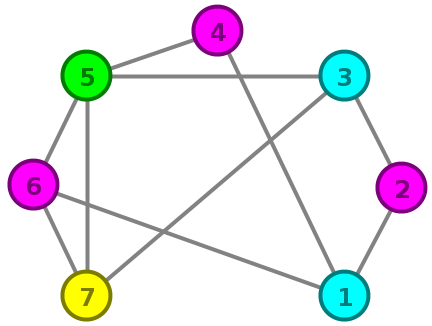
\includegraphics[width=0.45\linewidth]{bad_order_color}
   \hfill
   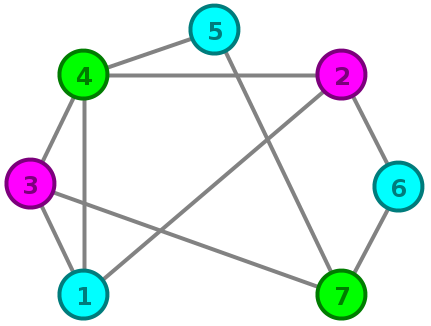
\includegraphics[width=0.45\linewidth]{good_order_color}
\end{figure}


\begin{figure}
\centering
   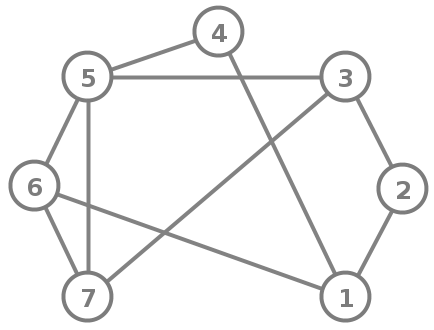
\includegraphics[width=0.4\linewidth]{bad_order}
   \hfill
   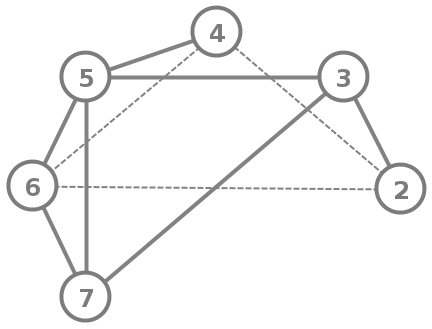
\includegraphics[width=0.4\linewidth]{bad_order_1_removed}
   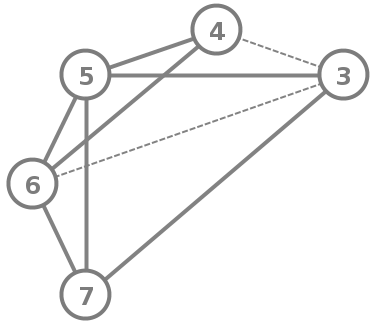
\includegraphics[width=0.4\linewidth]{bad_order_2_1_removed}
   \hfill
   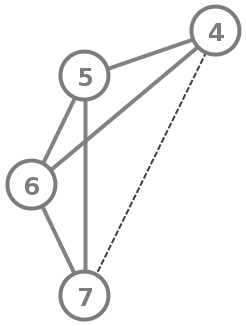
\includegraphics[width=0.3\linewidth]{bad_order_3_2_1_removed}
\caption{The bad  ordering}
\label{bad_order_fillin}
\end{figure}


\begin{figure}
\centering
   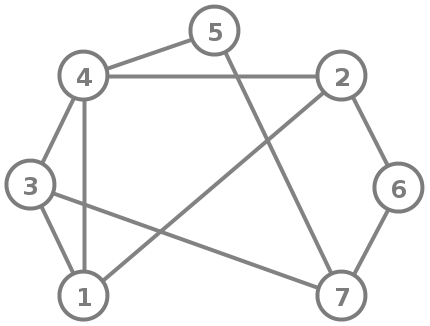
\includegraphics[width=0.4\linewidth]{good_order}
   \hfill
   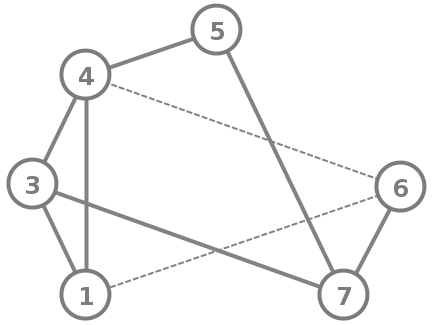
\includegraphics[width=0.4\linewidth]{good_order_2_removed}
   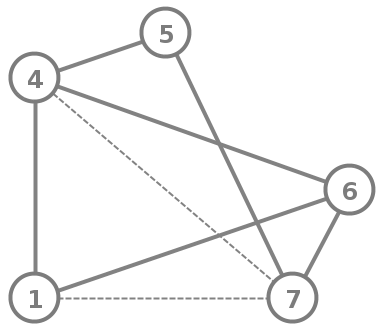
\includegraphics[width=0.4\linewidth]{good_order_3_2}
   \hfill
   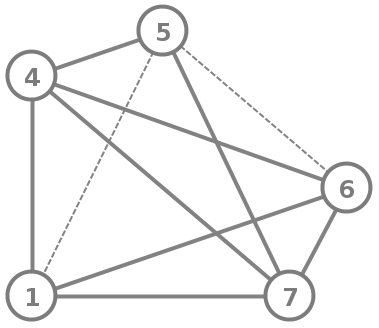
\includegraphics[width=0.4\linewidth]{good_order_4_3_2}
\caption{The good  ordering}
\label{good_order_fillin}
\end{figure}


\begin{figure}
\centering
   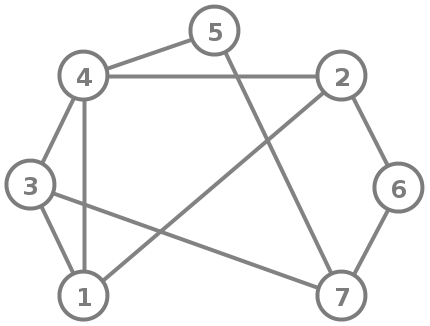
\includegraphics[width=0.4\linewidth]{good_order}
   \hfill
   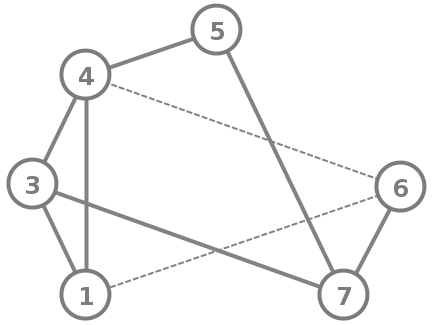
\includegraphics[width=0.4\linewidth]{good_order_2_removed}
   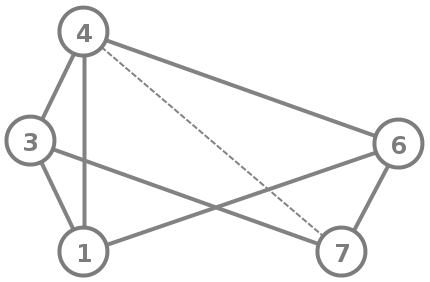
\includegraphics[width=0.4\linewidth]{good_order_5_2_removed}
   \hfill
   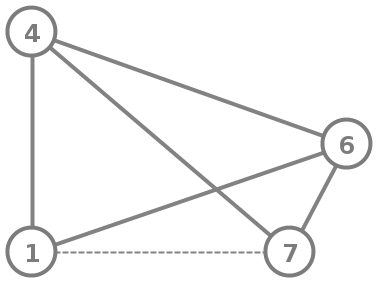
\includegraphics[width=0.25\linewidth]{good_order_3_5_2_removed}
\caption{The good  ordering}
\label{good_order_fillin}
\end{figure}














\chapter{Conclusion}
 
\bibliographystyle{IEEEtran}
\bibliography{refs}

\end{document}
